\chapter{Description logics and biomedical knowledge (Specification)}

\textbf{Key points}
\begin{itemize}
  \item Organisms can be compared to complex black box machines, namely devices with a hidden and unknown internal functioning.
  \item This analogy helps to define the study, needs and representation of biomedical knowledge.
  \item Description logics (DLs), part of a mathematical framework developed to formalise concepts, can be used to study the molecular black box machine and query over recorded biological knowledge. DLs provide the means to represent terms and logically link biological modules.
  \item The framework presented integrates with current life-science information, such as biomedical ontologies (OBO) and databases, and is theoretically highly scalable (\dl{EL\textsuperscript{++}} profile).
  \item The notions introduced and discussed set the groundwork for the representation of the mode of action and the implementation of a new resource built on these principles: The Functional Therapeutic Chemical Classification System (FTC).
\end{itemize}

\textbf{Author's comment}

This chapter is a summary and record of my experience with the Web Ontology Language (OWL2) and knowledge representation for the biomedical domain. I present a theoretical analysis of the representation of the mode of action and its scalable implementation. A software library to assist the development of programmatic solutions (Brain) is briefly presented in this chapter. I invite the reader to refer to the original publication \citep{croset2013brain} for more detail if wanted.

\hrulefill

\section{Introduction}

Science (from Latin scientia, meaning "knowledge") is a systematic enterprise that builds and organises knowledge in the form of testable explanations and predictions about the universe \citep{sciencewiki}. More specifically, biomedical sciences handle the subset of knowledge related to living organisms. Understanding the biological world is relevant to society as it provides, among other things, some valuable insight to treat and cure diseases. In order for our knowledge to grow, discoveries and evidence have to be recorded, structured and shared with the community and society. Traditionally, biological knowledge is preserved in a narrative fashion, inside textual documents, such as a journal article for example. However, natural language is ambiguous, informal, and impairs an efficient reuse of the information. More recently, with the advent of computer systems, some biological knowledge is stored in a structured way inside databases or ontologies \citep{brooksbank2014european}. Biological entities and concepts have identifiers, enhancing the dissemination and reuse of the information, as well as enabling an efficient integration of multiple datasets. Despite the improvements made towards a more meaningful and consistent representation, I argue that the "logic" in "biologic" is still under-represented. Indeed, it would be valuable to formally derive and prove new facts from existing ones, the same way it is done in algebra for instance. This chapter presents an original approach towards this goal, using description logics (DLs) as a mathematical framework.

In this regard, I first illustrate how the study of organisms is analogous to the theoretical study of a black box machine. From this simple fundamental model and its requirements, I then explain how DLs can, to some extent, capture the internal logic of the cellular machinery. Finally I discuss how this approach can be combined with existing biomedical data, in order to implement automated and scalable solutions. This theoretical work serves as the basis to formally define the concepts of mode and mechanism of action, central points in deriving drug repurposing hypotheses.

\section{Biomedical knowledge}

Life sciences addresses the study of living organisms. Just as in any other scientific discipline, biological researchers first collect data and evidence, which will then be turned into knowledge based on human interpretation \citep{antezana2009biological}. In order to be efficiently reused, understood and shared with the scientific community, some of this knowledge can be represented by a process known as formalisation.

\subsection{Contemporary formalism in biomedical sciences}

Formalism can be described as an abstraction process by the human brain in order to model a system in mathematical terms. Formalising a problem helps to better analyse its complexity. Mathematical models (e.g, equations) are powerful, as they can eventually predict outcomes, once the system is understood well enough. Different scientific disciplines employ different formalisms, depending on the problem studied and research questions being asked.

\subsubsection{Formalism varies among natural sciences}

\begin{figure}[ht]
    \centering
    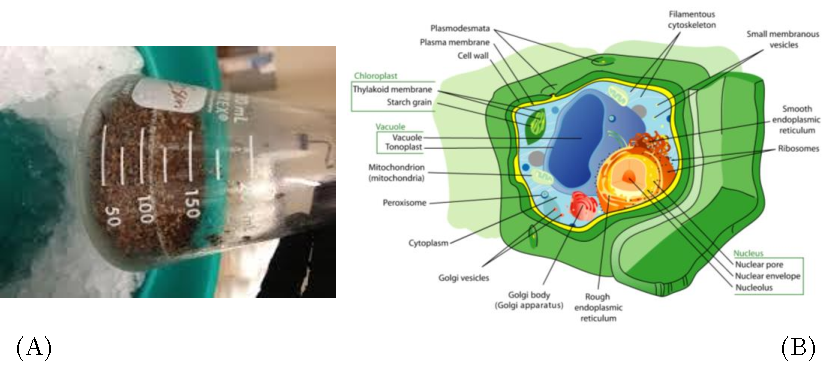
\includegraphics{fig2-1}
    \caption{Examples of capture of information in biology. (A) A flask containing hundreds of individuals of the species drosophila melanogaster. The population is identified with a label on the container. (B) Schema of a  canonical plant cell, similar to the one found in text-books. Parts of interest are annotated with terms, following a descriptive approach. Pictures from Wikipedia and courtesy of Sarah H Carl.}
    \label{fig2-1}
\end{figure}

When I was a college student, I always found biology to differ from other natural sciences such as chemistry or physics for instance. The latter disciplines were built around a particularly strong mathematical scaffold; fundamental phenomena, like the speed of a body, were concisely captured by a function such as $ v=d/t $. Chemical reactions were simplified in the form of an equation such as $ H_{2}O = HO \textsuperscript{-} + H \textsuperscript{+} $ for instance. Despite being approximations of natural processes, these models and equations were useful to learn the discipline. Moreover, once the core concepts were understood, some supplementary layers of complexity were logically added on the top of the known things: Static representations of chemical reactions were transformed into dynamic ones, or it was possible to derive the trajectory of a projectile from its speed and direction, for example.

The formal representation of a system is important, as it clarifies the meaning of the concepts of interest for the community. For instance, speed has a very explicit and clear definition captured by its equation, which can be unambiguously understood and interpreted accordingly. Finally, the most important feature of a formal system is, I believe, that it enables predictions to be made. It becomes possible to infer behaviours and results on the sole basis of the theory. Complex systems can be built and fully understood, relying solely on fundamental principles.

The study of biomedical sciences was not guided by such strong mathematics. Core concepts such as evolution or gene were mostly described in a textual way, a sentence usually defining the meaning; it was impossible to combine concepts in order to create new ones. As biological organisms obey the law of physics and chemistry, one would therefore assume that these frameworks could assist in the study of the living world on their own. They do to some extent; it is for instance possible to represent and model the series of chemical reactions related to a biological pathway using standard chemistry \citep{le2006biomodels}. However, biomedical sciences present particular challenges that cannot adequately be solved by the traditional molecular formalism. First of all, biological bodies are extremely complex from a chemical perspective, either in terms of size or types of compound present (3 x 10\textsuperscript{27} atoms in the adult body and a minimum of 25 atom types) \citep{nielsen1999ultratrace}. Secondly, some high level phenomena have an unknown molecular basis, and it becomes therefore impossible to capture formally the system while solely relying on chemistry. Phenotypes and diseases are good examples of this category.

Because of these obstacles among other things, biomedical sciences are traditionally less formalised than their counterparts, the biological knowledge being often captured by a textual description inside a document, or sometimes with the help of a conceptual schema \citep{lazebnik2002can}. Figure \ref{fig2-1} and \ref{fig2-2} present examples of media used to convey, record and communicate life sciences knowledge.

\begin{figure}[ht]
    \centering
    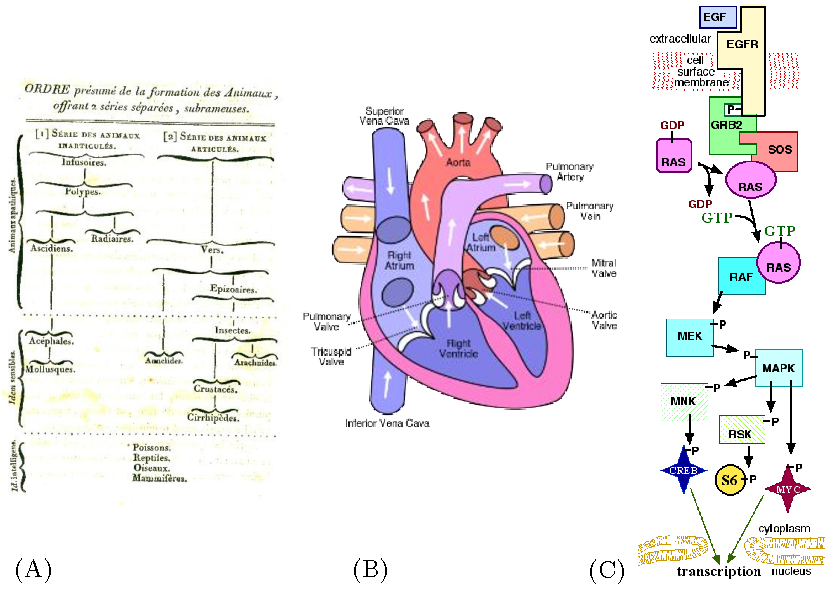
\includegraphics{fig2-2}
    \caption{Formalisation in biomedical sciences. (A) Diagram showing the evolutionary taxonomy of invertebrates. Drawn by Jean-Baptiste Lamarck's in 1815. (B) Mechanistic illustration of the cardiovascular system. Arrows illustrate the flow of blood and the logical connection between the annotated parts. (C) MAPK/ERK signaling pathway. Schema of the cascade of molecular events leading to activation of transcription factors. The logic of the system is informally captured using arrows, colours and shapes. Images from Wikipedia.}
    \label{fig2-2}
\end{figure}

Nowadays, with the advent of computers and the Internet, known biological entities and concepts are further stored inside public databases. Often, a manual curation step over the published literature improves the consistency and correctness of the data \citep{brooksbank2014european}. The structured information makes it easier for the community to retrieve the data and to perform statistical analyses on it. Nonetheless, this framework is not fully formalised; for example it is not possible to mathematically prove why a drug could be useful for a disease, such as one can logically derive with a series of steps the value of the variable $ x $ out of the following equation: $ 2x = 4 + x $.

How can one further formalise biomedical knowledge to assist the development of new medicines and the study of the living world? A naive approach would try to simplify the system life scientists are working with into a meaningful analogy \citep{lazebnik2002can}. In this regard, I will present how the study of a living organism can be compared to the study of a black box machine, namely a device for which nothing about the internal workings is known (see Figure \ref{fig2-3}).

\begin{figure}[ht]
    \centering
    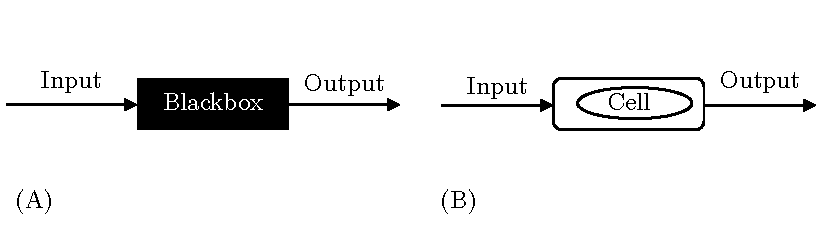
\includegraphics{fig2-3}
    \caption{Blackbox model. (A) Schematic representation of a blackbox. Given an input, an observable output is produced. The internal workings are supposedly not understood. (B) Cells or organism are blackboxes: They can carry various and observable functions from an input, yet the internal workings are not necessarily fully understood.}
    \label{fig2-3}
\end{figure}

\subsubsection{Organisms as complex machines}

From the perspective of drug discovery, an organism (related to organisation) can be broadly simplified as an assembly of molecules functioning as a stable whole. This characteristic makes organisms similar to a machine in the generic sense, which can be described as an assembly of parts functioning to meet a particular goal; in the case of the organism, the intrinsic goal is survival or reproduction. Based on these definitions, biomedical sciences can be seen as the sciences of preventing and repairing dysfunctioning organisms - or molecular machineries.

According to this analogy, the study of a living organism can therefore be compared to the study of a complex black box machine, composed of a large number of physical parts carrying a certain number of internal functions and acting together in an organised fashion.

Now assuming that a certain community has access to such a machine and wants to study it for various reasons, how can it theoretically be done? The analogy becomes insightful at this stage, as there are plenty of complex man-made devices the reader can relate to, and which will serve to illustrate the thought process. I will consider an airplane as example, because it is a complicated device with a straightforward goal: safely flying in the air. A similar exercise can be done with a radio \citep{lazebnik2002can}.

Supposing that a fully functional airplane was found somewhere and the only thing known about it was that the device is capable of flying. The aim is to understand as accurately as possible how the machine works, in order to have enough knowledge to be able to fix it in case it gets broken or malfunctions in the future. In order to address this problem, I argue in favour of a straightforward descriptive approach, in line with the way biological sciences are performed, namely describing the device in as much detail as possible.

The first task done would be to schematise the device, as shown in Figure \ref{fig2-4}-A. Then the fundamental physical parts would get annotated with arbitrary names (\ref{fig2-4}-B). With an increased understanding of the physical modules composing the airplane, it would then be possible to discover the roles played by the various parts of the machinery. Objects would receive functional annotations, namely an explanation of what they do in the overall flying process, as shown on Figure \ref{fig2-4}-C. Up to this step, the system would be characterised as a collection of discrete physical and functional modules, each isolated from one another. Finally, in order to appreciate the machine as a whole, it would become mandatory to link the modules based on their relation types. Figure \ref{fig2-4}-D shows the high level logical organisation of the machine, which integrates the parts to understand the overall process.

\begin{figure}[H]
    \centering
    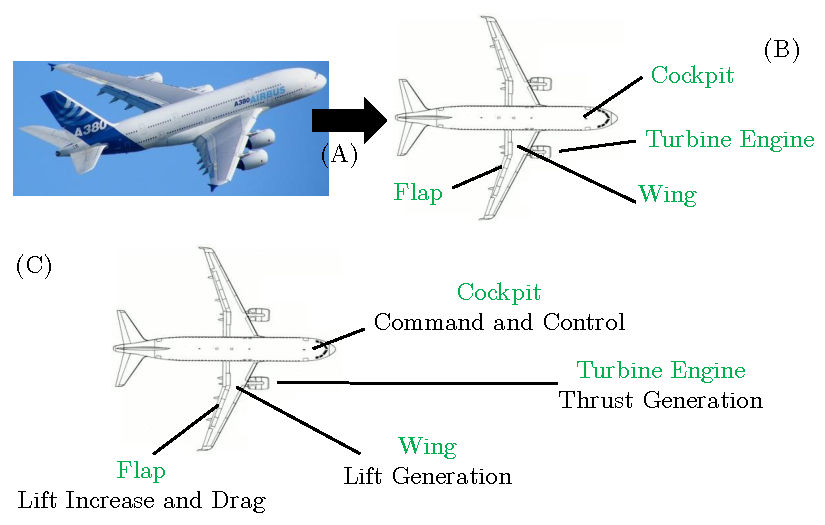
\includegraphics{fig2-4}
    \caption{Caption.}
    \label{fig2-4}
\end{figure}

Unveiling the internal logic of the black box machine using this descriptive methodology would later allow extensive querying of the model of the system and simulation of its behaviour. For instance, assuming a problem was identified with the lift of an airplane, preventing it from flying. From the model, it would be possible to retrieve all the known parts directly or indirectly involved in the lift process, derive a list of potentially faulty components and suggest ideas on how to logically repair it and restore its ability to fulfil its primary goal, flying.

The black box machine analogy allows one to better understand the requirements of a formal descriptive framework in order to capture biomedical knowledge. From a drug discovery point of view, organisms can be fundamentally reduced to machines. The descriptive process of studying such machines I presented is analogous to the approach researchers use to study organisms, understand diseases and find treatments for them.

In order to move from an informal characterisation into a defined framework, it is first necessary to determine what is required for a descriptive approach to successfully capture biology. The next section will identify some of the concrete needs for biomedical knowledge, derived from the theoretical model of the molecular black box machine and its study.

\subsection{Requirements for biomedical knowledge formalisation}

In order to be efficiently reused and shared, biomedical knowledge has to be formalised. One way to investigate the living world consists of considering organisms as complex machines; descriptions and annotations of the parts of the machine then help to represent the knowledge and understand better the functioning of the whole device. However, in order to be meaningful, this descriptive approach needs to fulfil a series of criteria introduced in the following section.

\subsubsection{Mathematical framework}
\label{reqmath}

Extending a mathematical field is a key feature of any formal framework. Mathematics help to accurately formulate problems and provide the generic means to solve them. In the case of biomedical knowledge, the ultimate aim is to reduce the burden of diseases for society. To achieve this goal, a formal framework must first be able to capture biological information. Secondly and more importantly, it should be possible to further exploit the framework to deduce and prove assumptions over it. For instance, the mathematical branch of geometry handles questions related to shapes and space. Even if this framework provides only a simplified view of reality, geometry provides the formal means to attest to the validity of a building's blueprints or optimise land exploitation. Similarly, in the biomedical domain, one should expect to be able to deduce implicit facts or formulate new hypotheses regarding potential treatments directly out of the mathematical formalisation, which is currently not the case. Connecting descriptive biomedical knowledge with mathematics also insures that the framework can benefit from the latest progress in the field. It helps different communities to work together on the same issues from different angles. Formulating biomedical knowledge in mathematical terms also opens the door for computer sciences to assist later on with the implementation of a digital solution.

\subsubsection{Definitions}
\label{reqdef}

The annotation of the parts of the machine requires the usage of a new and specific vocabulary. Words and concepts can be ambiguous, especially when the system analysed is complex such as a living body. A recent illustration of the importance of definitions in biology is the debate over the ENCODE project conclusions \citep{Form_and_function_2013}; different scientists have different interpretations of the word function, which shift the explanation of the results. Semantics, the investigation of the meaning of symbols and words, can assist in this task and help to specify the intended meaning of a concept. Moreover, a formal framework for biomedical knowledge should be able to define any type of things: real-life objects, such as molecule, protein or cell for example. Abstract biological processes like blood coagulation or diseases such as cancer should also be part of the framework, as they are essential concepts in biomedicine. Finally, in order to appreciate the logic of the machine as a whole, it is mandatory to be able to link concepts and words, in order to show how parts of the machinery interact together. The meaning of such relations should be explicit and unambiguous, just as the definitions of concepts.

\subsubsection{Hierarchies and abstraction}
\label{reqhie}

In practice, organisms are probably more analogous to Rube-Goldberg machines than airplanes (see Figure \ref{fig2-5}), with an internal logic sometimes difficult to understand on its own; this results in practice in a tangled network of chemical wiring, which can be abstracted and simplified into functional modules (\cite{hartwell1999molecular}, \cite{ravasz2002hierarchical}, \cite{machado2011modeling}, \cite{fisher2007executable}). Biomedical knowledge has to deal with entities ranging from chemical drugs to high level concepts such as species or biological processes. All these layers have to be integrated and linked in order to understand the machine as a whole. In this regard, it is critical for the formal framework to support abstraction and enable the representation of hierarchical information.

Taxonomies have always been at the heart of biological sciences; take for instance the work of Carl Linnaeus and the Systema Naturae \citep{von1770systema}. Classifications are further used to organize species, protein and chemical families, to name a few examples. Historically speaking, categorical information has provided a good and intuitive framework to capture biomedical knowledge; therefore, any attempt for further formalisation must be able to handle this type of data, as well as to leverage its use.

\begin{figure}[ht]
    \centering
    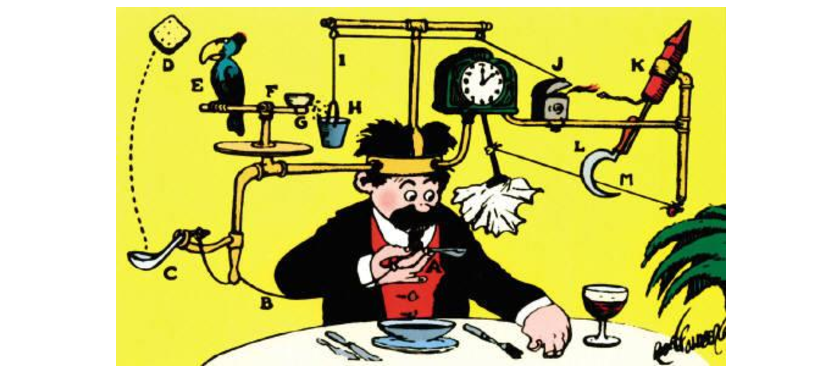
\includegraphics{fig2-5}
    \caption{Rube Goldberg machine: Over-engineered machine that performs a very simple task in a very complex fashion, usually including a chain reaction \citep{rubewiki}. The picture shows the "Self-Operating Napkin". When the spoon soup is raised, a cascade of events are triggered ending as the napkin coming toward the man's face. The task performed is relatively trivial, yet many steps are needed to execute it. Organisms are assumed to be analog to Rube Goldberg machines because of evolution; the internal wiring is not necessarily straightforward and progressively evolved and changed \citep{ravasz2002hierarchical}. Illustration from Wikipedia.}
    \label{fig2-5}
\end{figure}

\subsubsection{Distributed and scalable}
\label{reqscale}

Studying a system as elaborate as an organism requires the collaboration of a large number of persons, working in parallel on different facets of the problem. All these individuals must be able to access and share their knowledge, in order to communicate and be aware of the latest progress. Disseminating information has been usually performed via printed literature, which is being replaced at the time of writing by the World Wide Web and the Internet. This shift of infrastructure allows the processing of more and more information in a digital context, where computers can perform an increasing amount of the work in an automated fashion. This characteristic is particularly interesting for biomedical information, as it is possible to use computers as part of the formalisation process. However, this approach leads to challenges, in particular scaling issues. As organisms are of high complexity, it is therefore important to opt for a formal solution able to cope with problems of large input size. It is assumed that biomedical knowledge will only grow bigger with time, so a mathematical framework should take care of this concern, in order to be future-proof. Finally, it is supposed that biomedical knowledge is and always will be incomplete; in order to be powerful enough, the mathematical formalisation has to able to handle missing information.

\subsubsection{Molecular dynamism}
\label{reqdyn}

One of the characteristics of living forms is their dynamism; as organisms are made of molecules, they are subject to the laws of chemistry and molecular dynamics. Organisms can be defined in chemical terms as semi open systems \citep{meng2004modeling}, which emphasises a strong relationship with the environment. Formalisms coming from chemistry, such as conservation of mass \citep{masswiki} or thermodynamics \citep{thermowiki} can represent and solve such systems, yet they are not suited to handle more abstract concepts from the biomedical domain. An ideal formal framework for biomedical knowledge would appreciate the impact and interaction with the environment, yet this requirement is extremely challenging in regards to the number of chemical reactions to be considered \citep{meng2004modeling}. Moreover, the chemical formalisation strongly relies on kinetic parameters to capture behaviour, which makes them vulnerable to missing knowledge. Finally, another concern is the effect of chemical concentration in regards to the function. For instance, the action of a drug strongly depends on its administered dosage. Understanding in detail the biological machinery and deriving correct predictions out of it implies considering molecular dynamics.

Formalising biomedical sciences can be done using a descriptive methodology; this approach has been used since the origin of the field and is an intuitive way to represent biological systems and facts. I presented in this section the theoretical requirements deriving from the descriptive methodology and more generally biomedical sciences. The coming section illustrates how DLs can address some of these requirements in order to mathematically formulate and further use biomedical knowledge.

\section{Description logics for biomedical knowledge representation}

DLs are part of a family of formal languages used to represent the knowledge of a domain of interest. The plural form of the word logic indicates that a multitude of languages exist, each one of them characterised by a certain type of expressivity, as it will be seen later in this chapter. The framework evolved from semantic networks \citep{allen1982s} and inherited its current name around 1980 with the advent of computer systems. DLs are well characterised from a theoretical point of view and implemented in the Web Ontology Language (OWL), a standard supported by the World Wide Web Consortium (W3C). For these reasons and because they address most of the requirements presented before, DLs are an ideal mathematical framework that can be used to formalise some biomedical knowledge.

\subsection{Problems addressed by description logics}

According to Gruber, DLs help to specify a conceptualisation \citep{gruber2009encyclopedia}. In the case of life sciences, the conceptualisation is the molecular machinery, finding its specification being the task of the researcher. In this regard, DLs come with a series of tools to define words and concepts, and in particular their associated meaning or semantic. This feature allows terminologies to be built to describe the molecular black box machine. For instance, it is possible to capture the relative difference in meaning between these three following abstract biological concepts using DLs: positive regulation, negative regulation and regulation. This task appears trivial for humans, yet the main motivation behind DLs is to be able to express such things in an unambiguous and formal manner, in order to deduce less evident information later on. With DLs, the interpretation of the meaning of a concept comes from its relation to other concepts. For example, the concept mammal is more generic than the concept human; this is asserted in DLs by stating that every instance of human is also a mammal. The mathematical interpretation is that the set of humans is a subset of mammals. An is a relation could also be drawn between the two concepts if they were represented as nodes (see Figure \ref{fig2-6}). This feature enables DLs to unambiguously define the meaning of words from a mathematical perspective. It is also possible to define in a similar way the meaning of relations and to use them to represent the logic and wiring of the molecular machine later on. Taken together, these theoretical properties alone address the needs for a mathematical framework (section \ref{reqmath}), capable of handling definitions (section \ref{reqdef}) and abstraction (section \ref{reqhie}).

\begin{figure}[ht]
    \centering
    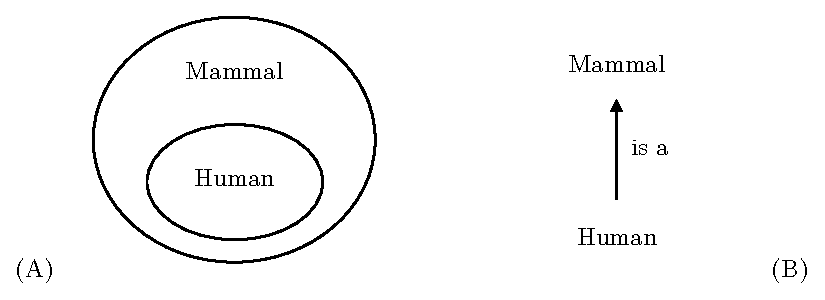
\includegraphics{fig2-6}
    \caption{Example of problem addressed by description logics. (A) The concept Human is more specific than the concept Mammal (all humans are mammals), which can be represented as embedded sets. (B) Same logic captured, representing the concepts as nodes and the relation as edge. The mathematical meaning of (A) (sets of instances) is more accurate than the meaning of (B), yet both representation can exist in practice, in particular in biology.}
    \label{fig2-6}
\end{figure}

The relations between entities and concepts are meant to formally express the known truth about a domain of interest (\cite{stevens2007using}, \cite{krotzsch2012owl}, \cite{hitzler2009owl}). This type of construct is called an axiom. A set of axioms constitute a knowledge base, also called ontology. The main interest of a knowledge base is the possibility to use the meaning of the axioms to deduce implicit things. Consider as an example the question, "What are the different types of mammals?" From the example before, Human would be logically deduced from the connection between the two categories (Figure \ref{fig2-6}).

From the formal representation it becomes possible to generate proofs and ask queries over the knowledge base; this operation is called reasoning and consists of two tasks: subsumption and consistency checking. Briefly the structure of the knowledge base arises from subsumption; concepts get classified into a taxonomy based on the axioms. Consistency checking can detect inconsistencies or contradictions that might be present in the knowledge base and report them. These services will be presented in details later in this chapter. It is important at this point to understand that the axioms of the knowledge base can be used to either generate more knowledge or to assess the validity of the current representation in a formal fashion. Reasoning tasks can be performed by humans and, more interestingly, by computers too. In fact, DLs have been developed for this very reason, to render domain knowledge computer understandable. The tight connection between computers and DLs is adequate for biomedical sciences, where it is expected to face large-scale data, beyond a sole human brain's capability to handle at once. The interoperability with computers makes DLs adequate to address the requirement for a distributed and scalable framework (section \ref{reqscale}).

DLs are efficient at representing terminologies and logical relations, yet they are unfortunately not appropriate to represent dynamic and temporal knowledge \citep{kim2008temporal}. This framework presents limits in regards to the molecular dynamicity requirement (section \ref{reqdyn}) and cannot handle well this facet of the machine. Work-around solutions will be presented later to the reader (Chapter 3).

Because DLs appear to address well a majority of the requirements for biomedical knowledge formalisation, I believe the framework to be suitable for the study of the molecular machinery. DLs can help to annotate and connect the logical parts in order to create a knowledge base, useful to understand the overall functioning of the system. Reasoning services allow for the querying and further use of the knowledge in a formal fashion, as expected from any mathematical framework. Finally the computer implementation of DLs is well studied, therefore part of the work can be automated, in order to come up with a scalable solution. Scalability guarantees the long-term success of the framework, but comes at the cost of expressivity.

\subsection{Expressivity and complexity}
\label{complexity}

Wikipedia defines expressivity as the breadth of ideas that can be represented and communicated. Let's consider for instance a molecule of methane; this concept can be represented in at least three different ways, more or less expressive and detailed, as shown in Figure \ref{fig2-7}.

\begin{figure}[ht]
    \centering
    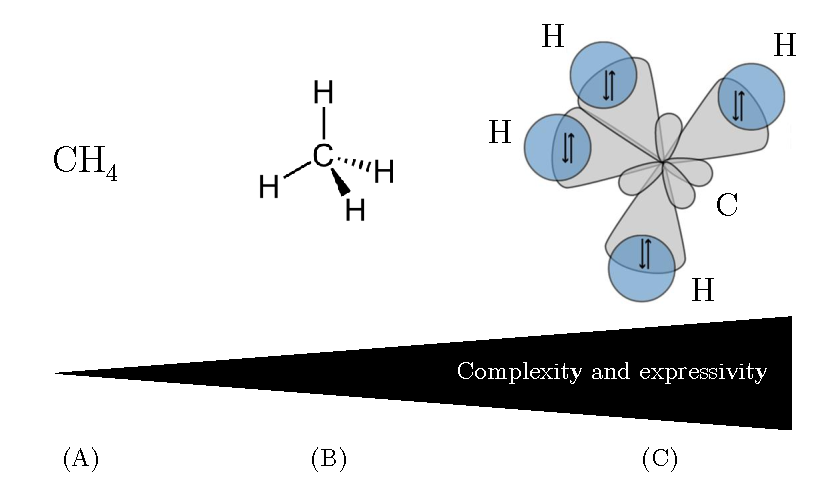
\includegraphics{fig2-7}
    \caption{Example of problem addressed by description logics. (A) The concept Human is more specific than the concept Mammal (all humans are mammals), which can be represented as embedded sets. (B) Same logic captured, representing the concepts as nodes and the relation as edge. The mathematical meaning of (A) (sets of instances) is more accurate than the meaning of (B), yet both representation can exist in practice, in particular in biology.}
    \label{fig2-7}
\end{figure}

What abstraction level is the correct one? It depends on the type of questions being asked on the model; all these three representations are legitimate and useful in practice for different purposes. The main difference between these models is their expressivity. Model \ref{fig2-7}-A for instance is less expressive than model \ref{fig2-7}-C; it conveys less detailed information, yet it is easier to understand and maybe more suited to study different types of problems. DLs are a family of logics, and just as with the methane molecule and depending on the type of axioms considered, they can model concepts in a more or less expressive fashion. As a rule of thumb, the more expressive the language is, the more complex it is. In the case of DLs, the complexity refers to the computational complexity, namely the time taken for the program to finish performing reasoning \citep{krotzsch2012owl}. The more axiom types are available to the user, the more time it will take to deduce their entailments. Complex problems are to be avoided in computer science as it will take more time to return a deduction from the content of the knowledge base, if a deduction is returned at all. This limitation comes from the hardware and the way computers are currently built (\cite{turing1950computing}, \cite{neumann1966theory}). In this respect, a scalable solution is a trade-off between expressivity and complexity. One would like to be as expressive as possible in order to study the molecular machine, yet able to deal with the very large input size of biomedical information. Fortunately, one of the strength of DLs is that their computational complexity has been particularly well studied (\cite{computationalprop}, \cite{ter2005completeness}). It is possible to work with a restricted set of axiom types, guaranteeing an acceptable complexity, appropriate for large-scale implementation. These fragments of DLs are also called profiles or subsets; one of them, the \dl{EL\textsuperscript{++}} profile, is particularly interesting for biomedical sciences (\cite{baader2005pushing}, \cite{baader2008pushing}, \cite{hoehndorf2011common}). I will focus in the rest of this chapter on this very fragment, as it is possible to reason over an \dl{EL\textsuperscript{++}} knowledge base in polynomial time. This characteristic makes reasoning tasks a tractable or so called easy problem \citep{cobham1965intrinsic}, which ensures that the framework can still work and scale for extremely large datasets. Despite offering a limited expressivity, the \dl{EL\textsuperscript{++}} profile provides the means to address a good portion of the requirements for biomedical knowledge formalisation, as will be presented in the coming section.

In the quest to formalising biological information, DLs have the very clear advantage of a well characterised computational complexity, ensuring the creation of realistic practical solutions with the help of a computer, and not theoretically limited by the size of the data. On the contrary, the computational complexity of simulating and modelling biological systems at the level of the chemical reaction is less neatly defined (\cite{meng2004modeling}, \cite{gillespie2007stochastic}) and appears much more complex and challenging; the fuzziness around the hardness of this task leaves an unanswered question as to whether modelling based only on chemical formalism will scale to systems as large as a cell.

\subsection{DLs' components and relation to life sciences}

Because of scalability concerns, it is wise to stay within the boundaries of relatively low complexity \ref{complexity}. To address that matter, I have presented the \dl{EL\textsuperscript{++}} profile as good candidate language, combining a decent expressivity for biomedical knowledge yet featuring constructs of an acceptable computational complexity. I will now present these constructs and components and explain how they relate to the life science domain. DLs are a theoretical framework and find a computer implementation as the Web Ontology Language (OWL2) \citep{owlw3c}. Despite being very close conceptually, these two frameworks have a few differences on the terminological level; I will therefore also mention the OWL2 equivalent names and symbols as a reference. OWL2 will be briefly discussed later in this chapter.

\subsubsection{Description logics core entities}
\label{coredl}

In order to represent the domain knowledge, DLs offer three kind of core entities, or building blocks: named individuals, roles and concepts. These entities are used to represent the world, and in this case, the components of the molecular machine. The first question that comes to mind is why these three types? The choice is purely arbitrary and likely derives from ancient Greece and the early work on categorisation done by philosophers such as Parmenides and Aristotle \citep{ontologywiki}. It appears that these three types can represent quite a lot of information, and they are fairly intuitive for humans to understand and reason over. They are an acceptable way to abstract the world around us.

\paragraph{\textbf{Named Individuals}\\}

OWL2 terminology: Individuals

The first building block handles individuals. Individuals refer to real-life instances and objects: this squirrel in a tree, this single molecule of water or glucose, this pen on a desk are all examples of individuals. Individuals are at the centre of DLs modelling. Everything else gravitates around them; all the further representation is done in regards to them. Every object can be considered as an individual.

Surprisingly, individuals are very rarely represented in life sciences. For example when one speaks about a particular protein, the reference is made towards the canonical version of the protein and not to the very one instance mixed with the millions of identical others. The same applies for diseases and species; the life scientist is concerned with extracting generic patterns and categories and reasoning at a more abstract level. This can be achieved by considering sets of individuals, so called classes or concepts.

\paragraph{\textbf{Concepts}\\}

OWL2 terminology: Classes

The second building block type handles concepts and terminologies. DLs concepts are interpreted as mathematical sets, namely groups of objects or individuals. Concepts represent an abstraction over instances and fit biological reasoning well. For example, the concept human contains at least two individuals, the reader and myself. Most biomedical ideas can be described as a concept (or class), including not only material entities such as molecules (e.g, P53 or Paracetamol) but also immaterial processes or functions (e.g, Blood coagulation or Catalytic activity). This characteristic makes DLs concepts very suitable to describe the molecular machine. The difference between an OWL class and its members is illustrated in figure 2-8-A.

\begin{figure}[ht]
    \centering
    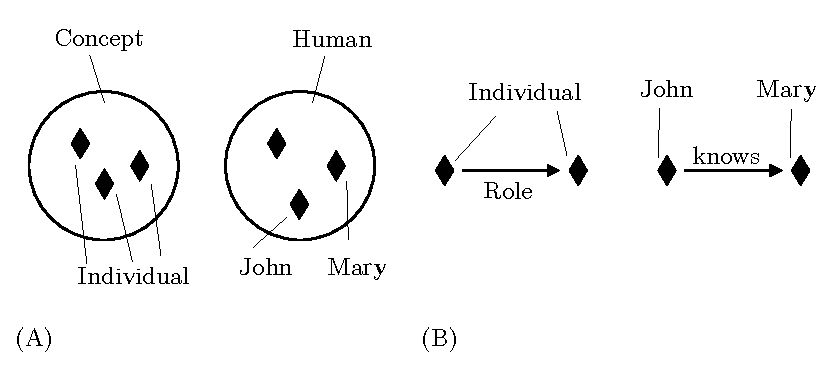
\includegraphics{fig2-8}
    \caption{Description logics core entities: (A) Concepts and Individuals: A concept or class is a set containing some individuals. On the example shown, Human is a concept, John and Mary are both distinct individuals. (B) Roles and Individuals: Role are linking two individuals. In the example, John and Mary are still individuals linked by the role "knows", specifying their relationship.}
    \label{fig2-8}
\end{figure}

\paragraph{\textbf{Roles}\\}

OWL2 terminology: Properties

The last building block deals with roles, namely how individuals relate one to another. Roles are more subtle and flexible to use than the two previous entity types. Basically they exist to capture a logical link between two individuals, and are so called binary in this respect (see Figure 2-8-B). In the study of the molecular black box machine, roles connect the modules and processes; they can represent the logical connections of the machine. Examples of roles commonly used in the biomedical domain are: regulates, part-of, involved-in, etc. Note that roles are only linking individuals; they cannot be used to directly link concepts.

\subsubsection{Axioms}

In DLs, the axioms are the reflection of our current vision of the world; they express the mathematical truth and help both humans and machines to interpret the meaning conveyed by the entities of the knowledge base (concepts, individuals and roles). Axioms enable deductions to be made. For instance, let's assume that there is an enzyme called thrombin which is somehow involved in blood coagulation (first axiom) and that a compound named ximelagatran affects the activity of thrombin (second axiom). From these axioms, one could conclude that the ximelagatran might logically affect blood coagulation. The progression from a set of axioms to a conclusion is called reasoning, and, as discussed previously, this operation can be performed by humans or by computers with the help of a program, called a reasoner. Different types of axioms exist, depending on what needs to be modelled.

\paragraph{\textbf{Assertional axioms (ABox)}\\}
The assertional axioms (or assertional box - ABox) are used to assert the truth about individuals. Although actual individuals are rarely represented as such in life sciences, it is still important to understand these fundamental types of axioms before looking at more complex ones.

\subparagraph{Concept assertion\\}
OWL2 terminology: Class assertion (or types). Concept assertion axioms link individuals to their concepts or types. For example, let's consider a knowledge base containing one named individual called john and one concept named Human. The axiom asserting that john is a human is written Human(john) or sometimes john : Human. It states that john is a member or instance of the class Human.

\subparagraph{Role assertion\\}
OWL2 terminology: Property assertion (or facts). This axiom captures the relationship between two individuals connected via a role. For example, consider two named individuals, john and mary, and a role, knows. Asserting the fact that john knows mary as shown in figure 2-8-B is written knows(john, mary) or (john, mary) : knows in DLs. Role assertions are sometimes said to create triples or sentences; this axiom type helps to render logical networks or graphs.

\paragraph{\textbf{Terminological axioms (TBox)}\\}

The terminological box contains the axioms related to concepts, which are therefore of primary interest for the biomedical domain. TBox axioms formalise the relationship among concepts in regards to the individuals they contain.

\subparagraph{Concept inclusion ($ \sqsubseteq $)\\}
OWL2 terminology: SubClassOf. Concept inclusion expresses the relationship between two concepts, one being more specific than or subsumed by the other. Assuming that there are two concepts, Human and Mammal, the concept inclusion axiom Human $ \sqsubseteq $ Mammal entails that all instances of Human are also instances of Mammal, or in other words all humans are mammals. Note that even if the assertion was based on a mental reasoning about individuals, in practice we do not see any individual names, only concepts. The axiom can be visualised in figure 2-9, alongside concept assertions.

\begin{figure}[ht]
    \centering
    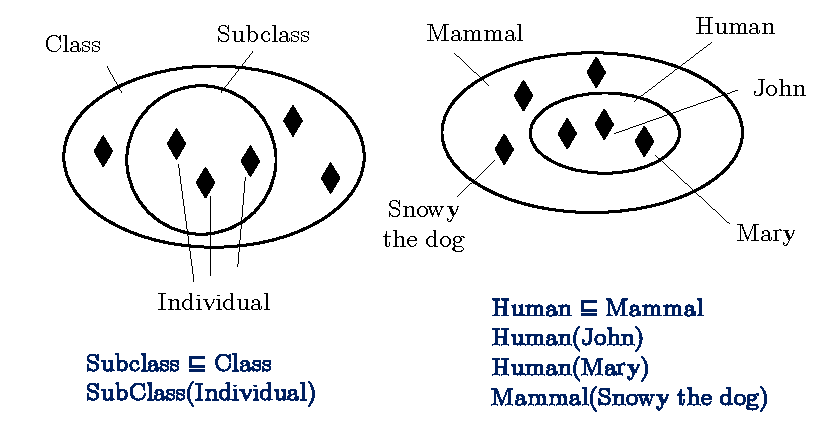
\includegraphics{fig2-9}
    \caption{Examples of description logics axioms, in blue with their graphical representation (concept assertions and inclusion axioms). Axioms specify the semantics linking the basic entities (individuals, concepts and roles). From a series of axioms or knowledge base, it is possible to deduce information. The question "What are the mammals present in the knowledge base?" would return as a result Snowy, but also John and Mary, even if they are not directly declared as such, from the semantics encoded in the axioms.}
    \label{fig2-9}
\end{figure}

\subparagraph{Concept equivalence ($ \equiv $)\\}
OWL2 terminology: EquivalentTo. It is sometimes interesting to define a set of individuals as equal to another set of individuals. This construct is mostly used to create new concepts from existing ones or to query a knowledge base. This axiom can state for example that the concept Human is equivalent to another concept or combination of concepts, as will be seen later in the chapter.

\paragraph{\textbf{Relational axioms (RBox)}\\}

The meaning of a role can be further specified in regards to the other roles of the knowledge base, in a similar way as is achieved with terminological axioms.

\subparagraph{Role inclusion ($ \sqsubseteq $)\\}
OWL2 terminology: SubPropertyOf. A role inclusion axiom defines the connection between two roles. Assuming that R1 and R2 are both roles in a knowledge base, and that the following role inclusion axiom holds: R1 $ \sqsubseteq $ R2, it means that all the time a pair of individuals is linked by the role R1, this pair is also linked by R2. The role inclusion axiom is analogous to the concept inclusion axiom for roles. A biological example concerns regulation: the role positively-regulates is subsumed by the role regulates: positively-regulates $ \sqsubseteq $ regulates.

\subsubsection{Constructors}

It is possible to specify the semantics of the core entities using axioms. The expressivity seen so far is however fairly limited. Fortunately the DLs constructors provide new means of expression as illustrated in the coming sections. Constructors allow for the composition of complex types from simpler ones analogously to how symbols of cuneiform scripts appeared to be used in some situations (see figure 2-10-A). Just as with axioms and entities, there are different types of constructors.

\begin{figure}[ht]
    \centering
    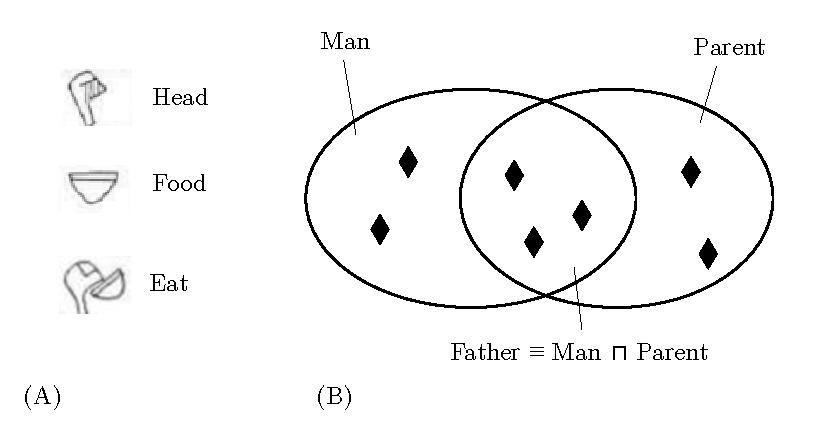
\includegraphics{fig2-10}
    \caption{Description logics constructors. (A) Constructors help to compose with concepts. The logic behind constructors is analogous to some of the semantic found in cuneiform scripts (3000 BC) (personal interpretation). (B) Concept intersection: The individuals member in the same time of the concept Man and Parent are asserted to be of type Father on the axiom presented.}
    \label{fig2-10}
\end{figure}

\paragraph{\textbf{Intersection ($ \sqcap $)}\\}
\label{intersection}
OWL2 terminology: Intersection (and, that)

The intersection constructor corresponds to the basic Boolean and operator used to describe overlapping sets. The figure 2-10-B depicts the meaning of the construct. An intersection can be used to formulate new expressions, which are used to create more complicated axioms. The concept Father can for example be expressed as being equivalent (equivalent concept axiom) to the intersection of the concept Man and Parent. Both conditions have to be true in order to satisfy this expression. From this axiom, assuming one knows that an individual is both a parent and a man at the same time, one could deduce that this individual is also a father. Note that because of the equivalence axiom, the concept Father is also inferred as being a subconcept of Man and Parent; indeed if an individual is a father, it is therefore a man and a parent too from our definition.

\paragraph{\textbf{Existential Restriction  ($ \exists $)}\\}
\label{exists}
OWL2 terminology: Existential restriction (some)

Existential restrictions encode a semantic subtle to grasp at first encounter (personal teaching experience). Yet they are particularly suited for the biomedical domain, as a means to link concepts via roles, something not doable with the constructs introduced previously. An existential restriction captures the fact that all individuals of a type X are necessarily linked by a property to some of the individuals of a type Y. For example, the expression $ \exists $ part-of.Cell refers to the sets of individuals that are necessarily part of a cell (see Figure 2-11-A). The presence of one of these individuals implies that here exists an instance of cell inside which they are located, no matter what. This expression can be combined with a concept inclusion axiom; for example, the concept Nucleus can be expressed as follows: Nucleus $ \sqsubseteq $ $ \exists $part-of.Cell. The axiom entails that a nucleus is something that is always part of a cell. But only being part of a cell ($ \exists $ part-of.Cell) does not necessarily qualify something to be a nucleus. Moreover, the axiom does not entail that all the cells have a nucleus. The example is represented and labelled in figure 2-11. Existential restrictions are very useful to represent biomedical knowledge; they allow one to link concepts with roles, without explicitly referring to specific named individuals. Their entitlements are not too strong and often adequate for the biological world.

\begin{figure}[H]
    \centering
    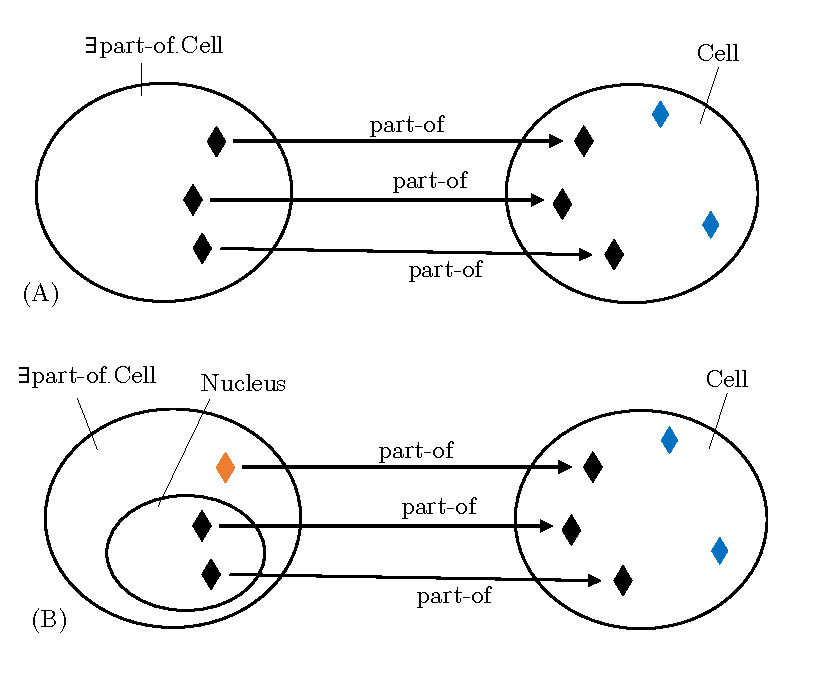
\includegraphics{fig2-11}
    \caption{Description logics constructors: Existential restriction (A) Example of existential restriction expression with the implication. Note that all individuals of $ \exists $part-of.Cell are linked to a cell individual via a part-of role. Yet some cell instances exist without being linked (in blue – for instance red blood cell). (B) Definition of the concept Nucleus from the existential restriction construct: Nucleus $ \sqsubseteq $ $ \exists $ part-of.Cell, meaning that all instances of nucleus are necessarily linked to an instance of cell. There exist some instances of $ \exists $ part-of.Cell not being nucleus instance (orange). This type of construct is commonly encountered in biology.}
    \label{fig2-11}
\end{figure}

\paragraph{\textbf{Role composition ($ \circ $)}\\}
OWL2 terminology: Chained properties (o)

The last constructor presented is the role composition. This construct enables chaining two roles together in order to create a new one. The typical scenario for this constructor is the "uncle" role, defined as a role inclusion axiom: brother-of $ \circ $ parent-of $ \sqsubseteq $ uncle-of. It is interpreted as if an individual X is the brother of a person with a kid, then X is the uncle of the child (see Figure 2-12-A). Closer to biology, an example of role composition is the expression regulates $ \circ $ part-of, which can be used to create the inclusion axiom: regulates $ \circ $ part-of $ \sqsubseteq $ regulates. This means that when the role regulates is followed by the role part-of, it could be simplified into a single regulates role. There is a special type of complex property inclusion called transitivity. It means that the role is chained with itself. For example: part-of $ \circ $ part-of $ \sqsubseteq $ part-of. The axiom is understood as if X is part of Y and Y part of Z then X is part of Z (see Figure 2-12-B).

\begin{figure}[ht]
    \centering
    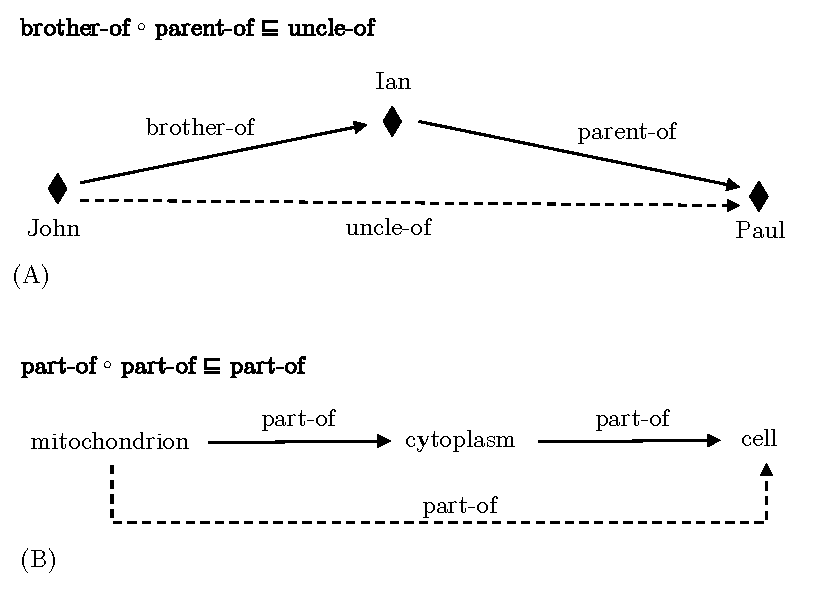
\includegraphics{fig2-12}
    \caption{Description logics constructors: Role composition. (A) Example of composed property, the "uncle" relationship. When two instances are linked using a "brother-of" property, then followed by a "parent-of" property, then a reasoner can create a property between the first and the last individual, as shown on figure between John and Paul. (B) Informal illustration of a transitive property using the Gene Ontology specification \citep{gorels}. When two terms are connected by a part-of relation and directly followed by another part-of property, then a part-of relation can be added between the first and last term. For instance here one can deduce that mitochondrion is part of cell, from the asserted facts. Note that this representation is not formal; OWL representation of OBO ontologies will be addressed later in this chapter.}
    \label{fig2-12}
\end{figure}

\subsection{Reasoning services}

Combining basic entities, constructors and axioms gives a knowledge base or formal representation of a domain of interest whose content can be handled by a reasoner. Considering the equation $ x + 2 = 6 $ as an analogy, axioms and entities helped to mathematically formulate the meaning of the symbols $ = $, $ + $ and $ 21 $; now a reasoner can automatically solve the equation and find the value of $ x $. In the biomedical case, the problem faced is different; the main task of the reasoner will be to classify the knowledge base and to answer queries about the functioning of the molecular machine.

As briefly mentioned earlier, reasoners perform two types of operations: subsumption and consistency checking of the knowledge base. I will not discuss consistency checking, as it is only meaningful if a certain type of axiom is present (disjunction axiom - not presented in this document, yet part of the \dl{EL\textsuperscript{++}} profile). The subsumption service is also called classification. In this context, it means assigning the right concept to the correct place based on the meaning of the axioms. Classified concepts form a taxonomy; for example the section \ref{intersection} explains how the concept Father can be asserted as equal to the intersection of the concepts Parent and Man. From this axiom, the reasoner can deduce that Father is subsumed by Man (all fathers are man), therefore Father can be classified as subconcept of Man and represented as such in a taxonomy (see Figure 2-13).

\begin{figure}[ht]
    \centering
    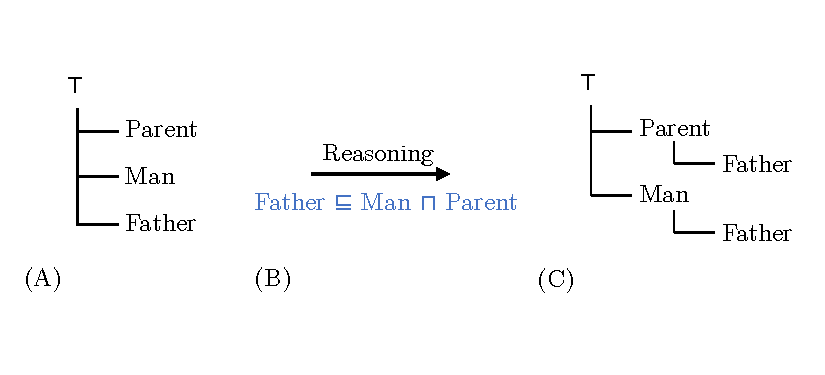
\includegraphics{fig2-13}
    \caption{Description logics subsumption service example. (A) Taxonomy of concepts not classified. (B) From the axiom present in the knowledge base Father $ \sqsubseteq $ Man $ \sqcap $ Parent (blue), the reasoning can deduce the taxonomy presented in (C). The concept Parent and Man subsumes Father, which appears deeper in the hierarchy, evidence of a more expressive meaning. The symbol $ \top $ represents the top concept (Thing in OWL) and is always present above every other concept of the knowledge base.}
    \label{fig2-13}
\end{figure}

The subsumption service is also responsible for answering the queries formulated over the knowledge base. A query is a standard concept expression. The list of concepts subsumed by the expression is the answer. DL queries are best orally formulated in the form of "What are the things that...". For example, "What are the things that are part of the cell?", expressed $ \exists $part-of.Cell in DLs. From the example of section \ref{exists}, the reasoner would deduce nucleus (see Figure 2-11).

The complexity of reasoning services depends on the types of axioms present in the knowledge base. The ones I have discussed here are part of the \dl{EL\textsuperscript{++}} profile, guaranteeing a tractable reasoning capable of handling large biomedical data input. Many more axiom types exists, featured by other DL families \citep{krotzsch2012owl}. Deductions over the knowledge base are performed by the reasoner, and can be simplified as a classification where the taxonomy of concepts is generated. 

\subsection{The Web Ontology Language 2 (OWL2)}
DLs are a theoretical mathematical framework. It is possible to manually exploit the meaning of axioms in order to perform reasoning services, but the goal is to eventually use a computer to perform this task, for time and data size concerns. In this regard, DLs are specified for computer implementation by the Web Ontology Language (OWL2) \citep{owlw3c}. OWL2 was primarily designed to help data interoperability over the World Wide Web and is tightly linked to the semantic web. Yet as OWL2 derives directly from DLs, it is possible to use the language to deal with DL-related problems, such as the study of the molecular black box machine. OWL2 terminology is slightly different from that of DLs, and the language provides some extra functionalities relevant to software implementation: concepts are called classes, and rather than having a human readable name such as Father, entities are identified with a Uniform Resource Identifier (URI), for example http://www.example.org/Father. This feature guarantees the provenance of the information, as domain names are unique in the World Wide Web \citep{berners2001semantic}. I will not discuss in details here the semantic web principles and design; the reader can simply consider that OWL2 enables the implementation of DLs in a computing setting.

One of the distinctive features of OWL2 is the open world assumption. This statement implies that nothing can be deduced from missing information. As an example: If the fact that drug A perturbs protein B is present and someone asks "Does drug A perturbs protein C?", the answer would be unknown. On the contrary, in a closed world setting such as relational databases the answer would be "drug A does not perturb protein C". The open world assumption fits the requirement of biomedical knowledge well; it is fair to assume that our knowledge of the living world will never be complete, therefore deductions can only be made over explicit evidence.

\section{Implementation with life-science information}

In summary, the theory presented previously states that DLs are a suitable theoretical framework for the descriptive study of biological organisms. The reader now might be wondering how an actual knowledge base is built using DLs. First of all, multiple implementations of the descriptive framework to study the black box machine can exist. The implementation of the theory varies depending on the questions asked and granularity required. Chapter 3 will present an example of implementation, made with a particular set of axioms, addressing the mode of action and drug repositioning. Other possible implementations could use other DLs features to characterise the black box machine to study other biomedical topics. However, in any case and in order to be successfully implemented in practice, this descriptive approach needs to extend the current solutions used to store biomedical data as much as possible. Reusing the information already available is beneficial as it decreases the amount of work to be done and allows for a non-disruptive transition from existing and adopted technologies. I will discuss here how the theory, namely the descriptive approach based on DLs, relates to current biomedical databases and ontologies - traditional keepers of the knowledge. Brain, a programmatic library dedicated to the OWL2 EL profile, will finally be introduced to show how scalable real-life applications can be built using DLs.

\subsection{Integration with biomedical ontologies}

\subsubsection{Open Biomedical Ontologies (OBO)}

In the early 2000s, with the advent of high-throughput DNA sequencing technologies, it became necessary to annotate genomes in a consistent fashion. The idea was to transfer the findings made in the sequences of one species to another organism. The Gene Ontology (GO) was first developed to address this problem \citep{ashburner2000gene} as a controlled vocabulary, representing molecular functions, biological processes and cellular locations. Following the successful adoption of the resource by the community, the Open Biomedical Ontologies (OBO) consortium was created, with the aim of creating a suite of orthogonal interoperable reference ontologies in the biomedical domain \citep{obofoundry}. OBO ontologies, usually contain synonyms of the described concepts as well as logical links between terms. It is encouraged to re-use the terms present in existing OBO ontologies, in order to create a net of biological concepts, sometimes called an integration layer. The OBO file format is traditionally used to serialise such ontologies (see Figure \ref{fig2-14}). This format provides a straightforward graph representation, similar to semantic nets, ancestors of DLs.

\begin{figure}[ht]
    \centering
    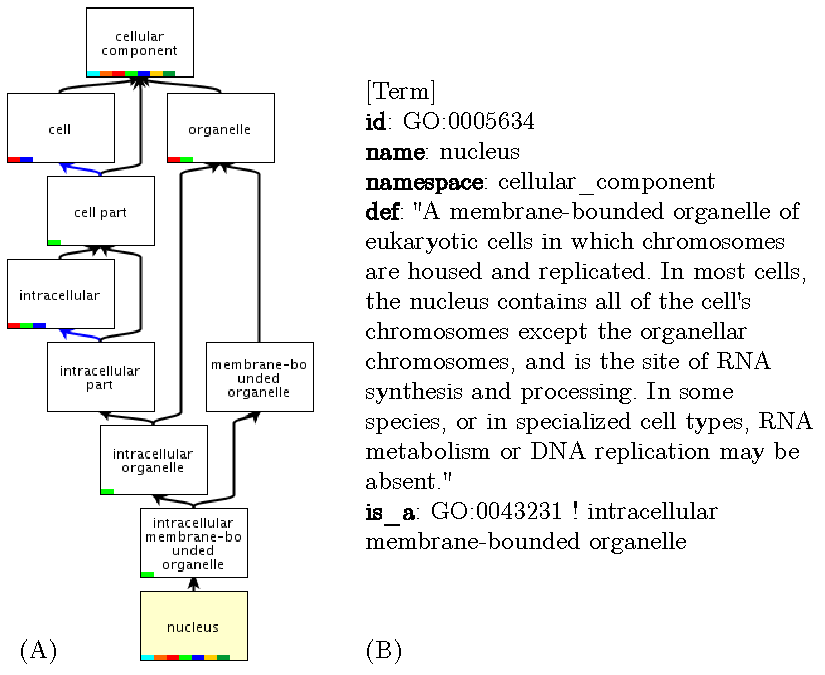
\includegraphics{fig2-14}
    \caption{Open Biomedical Ontologies format and representation. (A) The hierarchy above the term nucleus is presented. Black arrows entail an is a relation, blue ones a part-of relation. OBO ontologies are represented as directed acyclic graph. (B) Entry for the term nucleus, illustrating the format used to serialise OBO ontologies.}
    \label{fig2-14}
\end{figure}

The simplicity of the OBO format certainly helped the adoption of the standard by the community, yet it presents a limited expressivity with loose semantics, in particular from a computational perspective. Following the recent rise of semantic web technologies, the OBO community is currently considering a shift from the original OBO format into OWL2. Automated conversion from one representation to another has been extensively described in the literature \citep{tirmizi2011mapping} \citep{hoehndorf2010relations}. The main advantages in favour of adopting OWL2 are the possibility to reuse the numerous tools that have been developed as well as taking advantage of an extended expressivity to describe complex concepts.

The descriptive methodology presented in this chapter relates to the work done by the OBO community. First of all, as OBO semantics can be represented in OWL2, it is possible to directly reuse any OBO ontology to study the biological machine. Abstract concepts such as cellular functions or anatomical parts are extensively characterised inside some of the OBO ontologies and are therefore available to describe the parts of the cellular machinery. The main difference between OBO ontologies and descriptive knowledge bases comes from the lack of commitment towards interoperability and universality by the latter. Indeed, the reader will notice that I did not employ the word "ontology" to characterise the entity behind the study of the molecular machine. I purposefully avoided the use of the term in order to make clear that absolutely anything can be represented with DLs, as long as it serves somehow the study of a biomedical problem; the term "knowledge base" was used rather than "ontology" for this very reason. The main motivation behind the descriptive framework is to use computers and automated reasoning in an efficient, realistic and scalable fashion in order to derive biologically relevant information. Ontological commitment, in particular to top level concepts, entails the addition of complex axioms, which are hard to compute and most of the time outside of the OWL2 EL profile, such as universal quantifications for example \citep{krotzsch2012owl}. As a result, it becomes practically and theoretically impossible to use any reasoning engine over such an input size, defeating the purpose of representing information using an expressive language as OWL in the first place.

\subsubsection{Approximations and assumptions}

The biomedical ontology community is very eclectic, with representatives from various disciplines such as mathematics, computer science, philosophy and biology. Despite enriching the dialogue and improving the overall quality of the work resulting from this complex social network of people, it can also sometimes lead to animated arguments, pitting the vision of one branch of the community against another (personal experiences). Ironically, the ontology community cannot even agree on the meaning of the word "ontology" \citep{schulz2013formal}. In order to still make interesting usage of the powerful framework of DLs, I came to consider a set of rules of thumb, identified throughout my work, which will be briefly summarised in this section.

OWL and DLs can only define things arbitrarily. Just as in statistics, which are very popular in biology, the tests and data representation considered always depend on the type of questions to be answered, balanced with their computational complexity. It has been extensively argued that DLs are only relevant for a subset of biomedical knowledge, in particular to handle statements that are so called universally true \citep{schulz2013formal}, meaning true all the time, no matter what. Approximations are strongly discouraged in this mindset. I personally came to disagree with this argument; heuristics and approximations are present everywhere in biology. For example, the typical biological axiom considered as universal truth is the subconcept relationship between species \citep{schulz2013formal} \citep{krotzsch2012owl}.The concept Human is a subconcept of Mammal, meaning that every single human individual is also a mammal. A similar pattern can be applied across all other species. Any biologist will certainly agree that the boundary between two species is often fuzzy, as the main criteria used to distinguish them is based on the way organisms reproduce \citep{hanage2013fuzzy}. For some cases, such as mammals, it works rather intuitively well, but the approach is limited for some other species such as bacteria for instance \citep{hanage2013fuzzy}. This ambiguity is well known as the species problem and illustrates why it is impossible to simply clear cut two groups of living individuals in an ontological way while capturing evolution and biological meaningfulness. Another axiom widely considered as universal is the disjunction between the Male and Female classes, meaning that an individual cannot be a member of these two classes at the same time \citep{disjointw3c}. Such a statement, in addition to being socially offensive, also overlooks the complexity of the development of the hormonal system. Numerous existing individuals express sexual hormones in a dysregulated fashion (1/1000 births) \citep{dreger1998ambiguous}, leading to conditions such as hermaphroditism or gonadal dysgenesis. Their sexual anatomy therefore spans in between the typically expected sexual traits. Such cases are particularly relevant to medicine, yet a naive ontological separation between sexes would classify these instances as inconsistent and not handle them properly.

As shown, modelling complex systems such as biological organisms almost necessarily requires some approximations. Universality rarely holds in nature; I therefore argue that it is acceptable to represent biological approximations in order to tackle relevant problems of interest. The main motivation behind this deductive framework is the attractive possibility to use it in combination with a computer; this characteristic makes DLs unique and the focus should be put there. Biomedical axioms will most likely always be approximations, because of the underlying physical complexity of biological systems. By using the less restrictive term "knowledge base" rather than "ontology" I wanted to make this distinction: Biomedically relevant formal deductions can be made using DLs, and biological approximations can be represented. The rules of thumb to guide the representation I have adopted are the following:

\begin{itemize}
  \item Defining a series of competency questions. Such questions are the tests a reasoner should be able to deduce from a formal knowledge base. All the modelling resolves later to answer correctly these questions of interest. Approximations can be made, as long the assumptions are understood and interpreted correctly.
  \item Staying in the \dl{EL\textsuperscript{++}} profile, which guarantees scalability \citep{hoehndorf2011common}. Nowadays, the input sizes of interesting biomedical problems are too large for more expressive families such as OWL2 Full or OWL2 DL. Examples from the past show how a too expressive modelling fails to scale and give the promised answers in terms of reasoning \citep{vempati2012formalization} \citep{golbreich2006foundational} \citep{mungall2010integrating} \citep{mungall2011cross} \citep{villanueva2008yowl}.
  \item Trying to compromise between the constructs available inside \dl{EL\textsuperscript{++}} and biomedical approximations, in order to answer the competency questions.
  \item Not aiming for universality. It is of good practice to reuse and scale over the work done by other people, in the quest of interoperability (reusing terms, identifiers, patterns, etc.). However, the race for universality is much more challenging, as discussed before. I always advise designing knowledge bases to first answer the competency questions, and secondly, depending on time and energy, to maximise interoperability and aim for universality.
  \item It is to be assumed that deductions made over a biomedical knowledge base still require human interpretation. OWL and DLs are sometimes marketed (including by myself) as "knowledge discovery" tools; in practice the true discovery of new knowledge is made by a biomedical researcher, guided by the content of the knowledge base. A representative illustration of this argument is a figure featured on the original article introducing the gene ontology \citep{ashburner2000gene}, where the authors erroneously draw is a arrows linking terms in the opposite direction. Despite being semantically erroneous, the logic can be easily interpreted by any biologists, hence the success of the resource.
  \item Finally, I quote Hendler \citep{littlesemantics}: A little semantics goes a long way. This sentence is the motto of the semantic web movement and is widely accepted in the biomedical community too. By focusing on a few axioms, in particular on relational ones, a great and concise expressivity can be reached, as it will be shown with the definition of the mode of action presented in the coming chapter.
\end{itemize}

\subsection{Integration with databases}

As of 2014, a large amount of biomedical information is stored inside relational databases \citep{brooksbank2014european}. Some of this content is publicly available over the Internet, distributed by large organisations such as the European Bioinformatics Institute (EBI) or the National Center for Biotechnology Information (NCBI). Each database usually focuses on one theme in particular: for instance, ChEMBL \citep{gaulton2012chembl} provides millions of records about small molecules and their bioactivity against protein targets. These protein targets are themselves referenced inside Uniprot \citep{uniprot2013update}, a resource indexing the known information related to gene products. Records described in one place are moreover hyper-linked or crossed-referenced to records present in another resource, with the help of identifiers.

Biomedical databases can be seen as catalogues indexing the parts of the molecular machinery, yet not providing any logical information on how these entities connect. Interestingly, DLs provide the means to capture this logical layer, thanks to the expressive power of object properties. DLs can perfectly integrate with the information currently provided by biological databases, in order to enhance the semantics of the data. Consider the following scenario as an example: it is known from experimental evidence that a protein X is involved in blood coagulation, and a researcher would like to record this biological piece of knowledge. As of 2013, this statement is partially captured using the information of three repositories: Uniprot, the GO and the GO Annotations (GOA). The database Uniprot provides the identifier for the protein X, the GO gives an identifier for the term "blood coagulation", and finally inside GOA one would find an association (pairing) between protein X and "blood coagulation". From the DLs perspective, the same statement can be formally captured by an axiom: protein X subClassOf involved-in some Blood Coagulation. Here the logicless annotation or association between the protein and the biological process has been formalised into something more meaningful and expressive. The role "involved in" can indeed be combined with other roles in order to reflect the logic behind the biological system. This example shows how DLs can reuse the information already present and leverage the connectivity between concepts \citep{jupp2012logical}. I will present in the next chapter how these relations can be combined and structured to define the concept of mode of action and automatically classify drugs.

Converting the information from a relational database into OWL implies a change in the representation. Traditionally, database entries are considered as instance records, belonging to a table or schema. This fact implies that a record, such as protein X as available in Uniprot would correspond to an instance or individual in DLs (section \ref{coredl}). However, in practice, billions of copies of this canonical protein X exist. Therefore when biological entities or concepts are modelled in OWL, instances often become classes. This representation is closer to the reality and should simplify the modelling and connection with other concepts, like molecular functions. However, it is perfectly acceptable to represent proteins as instances too in my opinion, depending on the type of question being asked over the knowledge base.

\subsection{Brain library - implementing programmatic solutions}

Successfully implementing a knowledge base requires a compromise between scalability and expressivity. I argued in favour of the \dl{EL\textsuperscript{++}} profile, providing an adequate expressivity for biomedical sciences and enabling tractable reasoning. The discussion so far was mostly focused on the theoretical aspect, yet in order to be used in a programmatic way, a library or programmatic framework is needed. At the time of writing, two main free and open-source solutions exists to work with the OWL2 EL profile: Protege \citep{knublauch2005protege} and the the OWL-API \citep{horridge2011owl}. Protege is a popular graphical user interface, useful to develop toy examples and define the core axioms of a knowledge base. However, it is not very suitable for large knowledge bases, where potentially thousands of classes need to be handled. A programmatic alternative is a Java-based library called OWL-API. The framework implements the standard specification for OWL2 in deep granularity, yet it becomes quickly cumbersome to work with it in order to perform analyses and run biomedical queries. For these reasons, I developed Brain \citep{croset2013brain}, a Java library bridging the gap between these two solutions. This work is freely available online (https://github.com/loopasam/Brain) and open source. The library features a simplified interaction with DLs and OWL2 axioms using the Manchester syntax \citep{horridge2006manchester}. Figure 2-15 shows an example of a program written with the library.

\begin{figure}[ht]
    \centering
    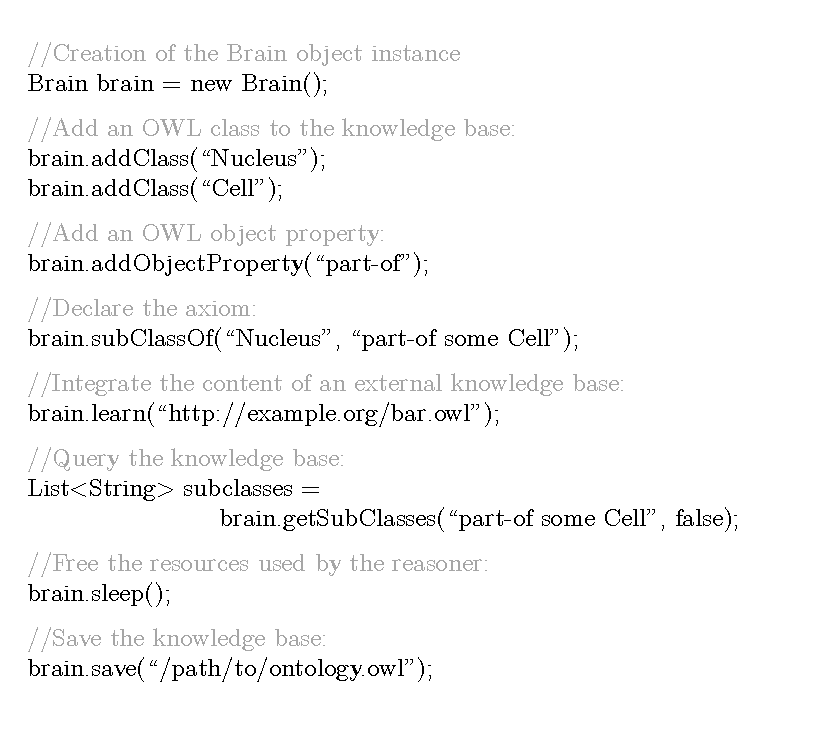
\includegraphics{fig2-15}
    \caption{Example of Java program written using the Brain library. Each command is preceded by a comment explaining the functionality.}
    \label{fig2-15}
\end{figure}

Brain uses the ELK reasoner \citep{kazakov2013incredible} to perform reasoning services over the knowledge base. ELK is dedicated to the EL profile, fast \citep{gonccalves2013owl} and can perform reasoning tasks in parallel; these characteristics make it an ideal candidate to handle biomedical knowledge. The Brain library mostly focuses on querying the underlying knowledge base; in this regards, OWL queries can be formulated as string expressions, which will then get automatically converted into Java objects and processed by the reasoner. Web applications can be safely built over the framework, as special care was put on thread management and coordination. Brain provides as well a series of convenience methods, useful to address biomedical questions; indeed, biological inference often derives from similarity metrics, such as sequence comparison \citep{stevens2007using}; the taxonomic structure of a knowledge base can also be used to derive a closeness index, so called semantic similarity, reflecting how close two entities are in the classification. The convenience methods provided by Brain calculate the Jaccard index over the set of superclasses. An illustration of the methodology is depicted in Figure 2-16. This type of analysis is out of the scope of DLs, yet particularly important for generating and exploring drug repurposing hypotheses, and will be further discussed in the coming chapters. The library offers the possibility to export graphs of the knowledge base, as exemplified by Figure 2-17. This functionality comes in handy to build web applications and to present content to users. Finally the reader might be interested by Tawny OWL \citep{lord2013semantic}, a similar application released approximately at the same time as Brain and with similar goals, but written in Closure.

\begin{figure}[ht]
    \centering
    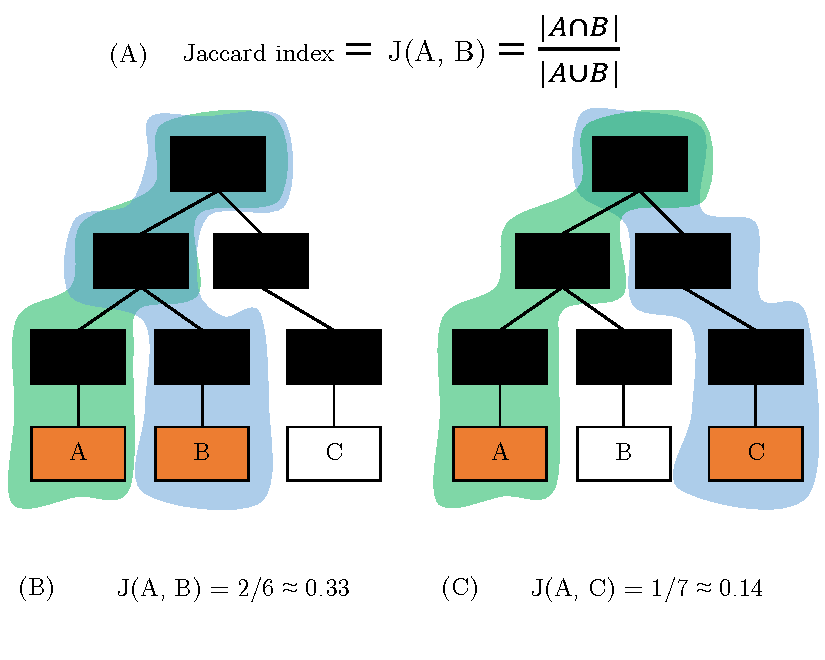
\includegraphics{fig2-16}
    \caption{Jaccard coefficient implementation in the Brain library alongside examples. (A) Definition of the coefficient: The similarity between two entities is defined as the ratio of the categories in common divided by the total number of categories. (B) and (C): Examples of computation of the index over two pairs (letters and in orange). The taxonomy is in black, super-classes shown with the blue or green area. The index is higher between the pairs A and B (0.33) than between the pair A and C (0.14), representing the fact that A and B are closer in the taxonomy and have a more similar meaning.  The coefficient will be used greatly later to compare the function of drugs.}
    \label{fig2-16}
\end{figure}

\begin{figure}[ht]
    \centering
    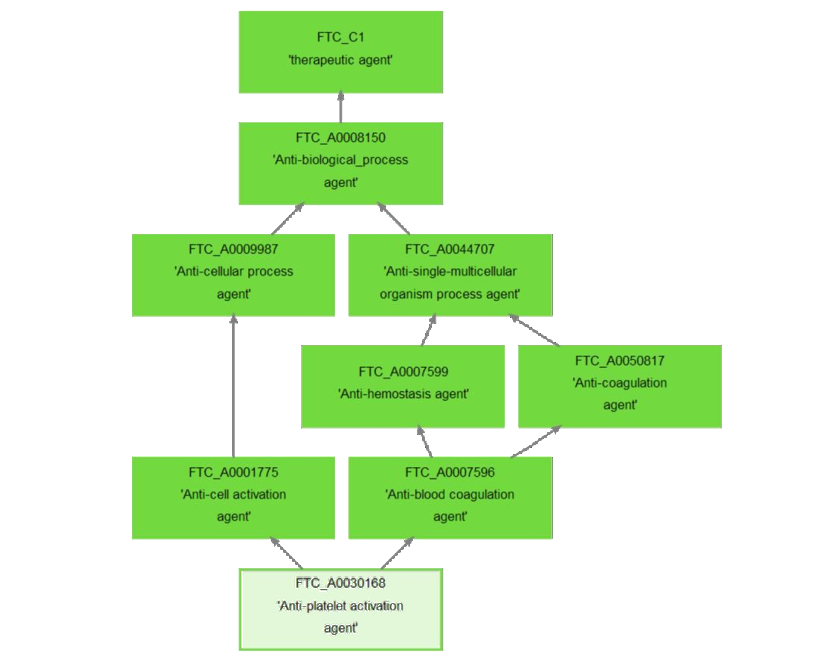
\includegraphics{fig2-17}
    \caption{Example of graph generated from the Brain library (content not pertinent): From an input concept, it is possible to export the whole ascendant taxonomy as scalable vector graphics (SVG), particularly useful to display information on web browsers.}
    \label{fig2-17}
\end{figure}

\section{Summary}

Living organisms are complex, yet understanding their internal machinery is required in order to develop new therapies and find treatments for diseases. Despite being eventually only made of chemical interactions, biological systems can be best analysed at a higher abstraction level. I presented how the study of life and resulting knowledge can be formalised using DLs. The main advantage of this framework is the possibility of defining abstract concepts (e.g, processes or phenotypes) as well as real entities (e.g, proteins or metabolites) in order to query or derive information using a computer. The logical links between modules of the cellular machinery can be modelled, and, computing their entailments resolves to a classification problem. DLs are less precise than molecular modelling, yet it is possible to derive formal solutions while considering the cellular system as a whole.

This approach integrates and leverages nicely the current information, available in resources such as databases and ontologies, in order to derive practical implementations. The analogy cell-machine will serve as the theoretical basis to formally define the concept of mode of action and address drug repurposing questions, as I will show in the next chapter and as summarised in Figure 2-18. Scalability was a core concern, in order to implement robust application. In this regard, I discussed the \dl{EL\textsuperscript{++}} profile, designed and inspired by the axiom types found in biomedical ontologies like SNOMED and guaranteeing the implementation of realistic solutions.

\begin{figure}[ht]
    \centering
    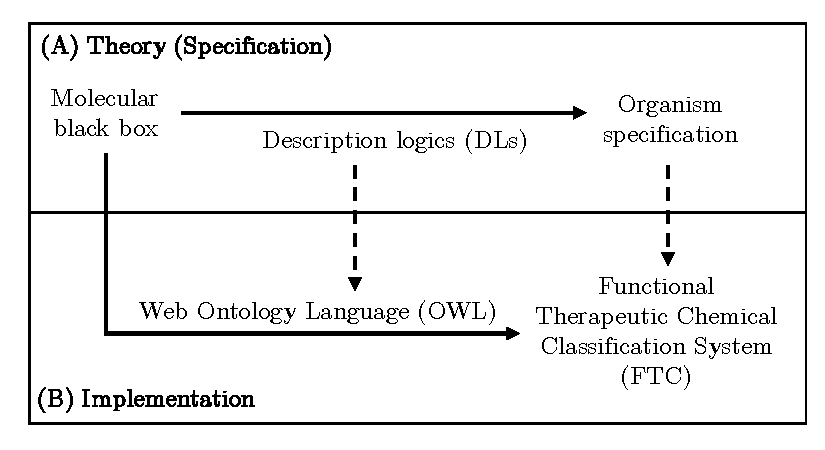
\includegraphics{fig2-18}
    \caption{Summary of the molecular black box theory. (A) To address drug discovery, organisms can be compared to black box machines. Description logics are a useful framework to unveil the specification of the black box machine. (B) The theory can be implemented (dashed arrow) for computers using the Web Ontology Language (OWL). Chapter 3 will present an example of implementation of the theory with the Functional Therapeutic Chemical Classification System (FTC), dedicated to handle the concept of mode of action and suited to repurpose drugs.}
    \label{fig2-18}
\end{figure}
